\documentclass[11pt]{article}

% use the free version of the Arial font
\usepackage[scaled]{uarial}
\renewcommand*\familydefault{\sfdefault} 
\usepackage[T1]{fontenc}
% so installing arial gives problems for wsl running texlive
% switching over to just using helvetica to get around that issue
% \renewcommand{\rmdefault}{phv} % Arial
% \renewcommand{\sfdefault}{phv} % Arial

% pandas tables
\usepackage{booktabs}

% figure wrapping
\usepackage{wrapfig}
\usepackage{graphicx}
\graphicspath{ {./images/} }

% text box
\usepackage{amstext}

% set margins to be 0.5 in
\usepackage[legalpaper, portrait, margin=0.5in]{geometry}

% set all font sizes in this document to be size 11pt
\renewcommand{\tiny}{\normalsize}
\renewcommand{\footnotesize}{\normalsize}
\renewcommand{\small}{\normalsize}
\renewcommand{\large}{\normalsize}
\renewcommand{\Large}{\normalsize}
\renewcommand{\LARGE}{\normalsize}
\renewcommand{\huge}{\normalsize}
\renewcommand{\Huge}{\normalsize}

% indent 1st paragraph
\usepackage{indentfirst}

% make references clickable
\usepackage{hyperref}

\begin{document}

\noindent
\textbf{Name:} Chinmay Raut \textbf{Dissertation Advisor:} Elizabeth Speliotes

\noindent
\textbf{Relevant Faculty: } 

\section*{Preliminary Exam (Specific Aims)}

Metabolic syndrome (MetS) is a combination of 5 health risk factors, including abdominal obesity, high blood pressure, high triglycerides, low high-density lipoprotein (HDL) cholesterol, and high fasting blood sugar, that together increase the risk for cardiovascular disease, type 2 diabetes, stroke, and other chronic conditions \cite{pmid29480368}. MetS diagnosis is based on thresholds for these 5 quantitative traits, and individuals must surpass the thresholds on 3/5 of these traits for diagnosis making this a complex disease to study. Up to 1 in 3 Americans currently satisfy the MetS conditions making it a significant public health challenge \cite{pmid29480368}. The underlying mechanisms of metabolic syndrome are not fully understood but are thought to involve a genetic component with MetS having an estimated heritability of about 20-30\% \cite{Graziano2019}. There is a need for further research to determine the underlying causes of MetS and to develop effective strategies for prevention and treatment.

Previous studies have identified hundreds of associations between common genetic variants and MetS using Genome-Wide Association Studies (GWAS) on databases of up to 300,000 individuals \cite{pmid31589552}. However, little is known about the effects of rare variants on MetS, and no large-scale ($>$100,000 individuals) rare-variant associations have been conducted on MetS \cite{Lee2018}. Rare genetic variants (minor allele frequency $<$0.05) are worth studying for three reasons: they make up most of the sites of variation across the genome \cite{pmid34662886}, they are predicted to result in significant phenotypic changes if they reside in protein-coding regions \cite{pmid34662886}, and studying effects in protein-coding regions also provides a direct route for future functional studies and therapeutic targets \cite{doi:10.1056/NEJMoa2117872}. With the integration of Next-Generation Sequencing and longer read technology, genetic repositories like the UK Biobank (UKBB) recently released their Whole Exome Sequencing  (WES) data (26 million variants across 450,000+ individuals) resulting in high-quality data on low-frequency genetic variants \cite{pmid34662886}. Currently, studies on rare variants in GWAS are limited by power due to low sample counts of individuals within a selected rare variant. A series of approaches have been developed to combat these limitations including the construction of the optimal Sequence Kernel Association Test (SKAT-O) \cite{pmid22863193} which combines a set of rare variants together to increase the power of the association test. When the SKAT-O test is paired with a variant annotator like the WGS Annotator (WGSA) \cite{pmid26395054} this results in the direct implication of genes to an outcome.

To understand the role genetic variants have on MetS, we want to identify and study its associations with rare, protein-coding variations using data from Biobanks. Exonic variants have the potential to alter proteins which then directly affect MetS phenotypes. Therefore, studying protein-altering variants offers direct insight into the biological mechanisms of MetS. We hypothesize that using WGS and WES data from large Biobanks such as the UKBB, we can detect exonic variants resulting in protein-coding changes which affect MetS. This will establish a series of protein-altering variants that provide insight into factors of MetS either for improvements in genetic testing or follow-ups for functional studies to investigate the biological mechanisms underlying the associations.

\subsection*{Aim 1: Determine Novel Gene-Based Associations with MetS.}

\textbf{Aim 1a: Identify genes associated with components of disease.} To avoid the issue of identifying single risk factor associations, like hyperglycemia associations, we can focus on the 10 (5 choose 3) distinct trait combinations for disease qualification. Using support vectors we will quantify an individual's disease severity score against each of these 10 combinations. We then run gene-based analysis techniques such as the SKAT-O tests to identify associations between genes and each of these MetS components.

\textbf{Aim 1b: Integrate discovered signals across components to study the holistic effect on disease.} After identifying significant genes across the 10 trait combinations, we will conduct enrichment analysis on the gene-based results from Aim 1a genes associated with multiple MetS profiles. We will also perform gene-based association tests against a joint severity score across the different trait combinations.

Based on the rare exonic variants we expect to identify and implicate specific genes that associate with components of MetS. We expect to construct a network of how these genes affect MetS as a whole, and if certain genes share similarities in effect on MetS providing further insights into its genetic basis.

\subsection*{Aim 2: Determine sequence-specific mechanisms of disease and progression.}

\textbf{Aim 2a: Within a gene, identify loci of individual variants affecting MetS.} We will perform Leave One Variant Out (LOVO) studies on the effects of variants within an implicated gene to understand if the effects of the protein-altering variants are restricted to a specific region of the gene or not.

\textbf{Aim 2b: Design CRISPR CAS9 KO guides based on exonic variants.} Based on the specific type of rare variants identified (frameshift, splicing, missense, etc…) we will design a CAS9 guide library surrounding those regions to study the functional effects of the identified variants in vitro.

We expect to produce a series of specific genomic loci potentially responsible for changes in MetS along with a CAS9 library for future functional experiments. This provides a direct target for future studies regarding the effects of genetic modification on MetS.

\

By studying new next-generation sequencing data to understand the role of rare genetic variants on MetS, we expect to identify genes that affect MetS and also provide biological insight into how they relate to the components of the condition. This study would lay the groundwork for further functional tests to investigate the biology behind the genetics of MetS and provide a genetics-based informatory tool to understand how one's genome contributes to risks in MetS.

\newpage

\subsection*{Background and Motivation}

Metabolic syndrome (MetS) is a combination of 5 health risk factors, including abdominal obesity, high blood pressure, high triglycerides, low high-density lipoprotein (HDL) cholesterol, and high fasting blood sugar, that together increase the risk for cardiovascular disease, type 2 diabetes, stroke, and other chronic conditions. ~33\% of Americans currently satisfy the MetS conditions making it a significant public health challenge. The underlying causes or biological processes behind MetS are not fully understood but the disease is thought to have a genetic component with a heritability estimate of 10-30%. 

Genome-wide association studies (GWAS) are a powerful approach used in genetics research to identify genetic variations associated with complex diseases or traits. In a GWAS, researchers analyze the genetic information of large groups of individuals to identify genetic markers, or locations along the genome, that are associated with the disease or trait of interest. By comparing the frequency of these genetic markers between individuals with the disease or trait and those without, researchers can identify specific genetic variations that may relate to the development of the disease or trait. GWAS for MetS have identified a couple of promising candidate genes such as APOB, LPL, CETP, APOA5, GCKR, and ZNF259 to be associated with MetS incidence in large European populations (>300k individuals). These genes implicate lipid metabolism to be a major contributor of MetS. However, since 2 of the defining characteristics for MetS are defined by lipids (HDL and triglycerides) and these genes have a lesser impact on the other 3 characteristics of the disease, it suggests that these genes alone do not explain the entire genetic effect on MetS.

\begin{wrapfigure}{r}{0.6\textwidth}
  \begin{center}
    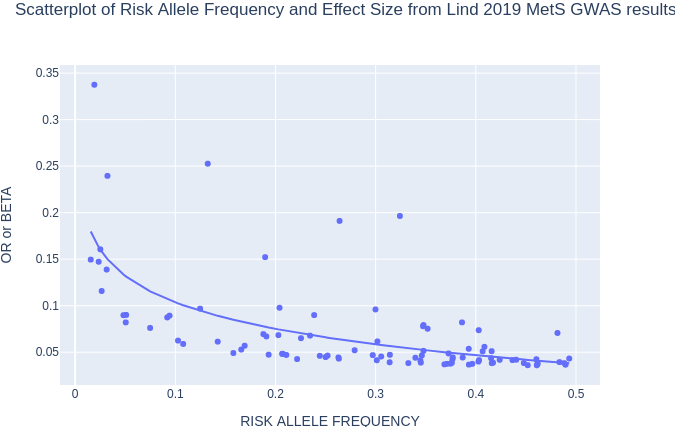
\includegraphics[width=0.60\textwidth]{"images/fig1v2.png"}
  \end{center}
  \caption{\textbf{Scatterplot of Risk Allele Frquency and Effect Size} (reconstructed from Lind 2019 MetS GWAS results). Effect size of variant increases inversely to allele frequency.}
  \label{fig:f1}
\end{wrapfigure}

Another limitation of most GWAS on MetS is that they are unable to detect associations between rare variants, defined as having a frequency of less than 1\% in the population. Previous studies tended to focus on common variants as this data is easier to acquire and study due to their increased imputation accuracy and prevalence in a population. However, one trend that has been identified through multiple GWAS is that rarer variants tend to have much larger phenotypic effects on an individual \ref{fig:f1}. There is potential that some of the large individual effects of genetic variants on MetS can be discovered through rare variant analyses. The primary problem of detecting rare variant associations lies within the rare nature of the variants. By definition, individuals with a selected rare variant make up less than 1\% of the population leading to massive sample size imbalances across carriers of a mutation vs non-carriers during the statistical tests. An alternative approach is to pool the effects of multiple rare variants, that we expect to behave similarly, together to combat the poor sample size imbalance. If we combine people that have any of multiple rare variants in an area we might have less imbalance of carrier vs non-carrier. One approach to this technique is known as the Optimal Sequence Kernal Association Test (SKAT-O). Most rare-variant associations use the SKAT-O in conjunction with variant annotation tools to test groups of variants belonging to the same gene or genomic region to directly implicate new genes with outcomes instead of specific point mutations. 

Advancements in sequencing technology have resulted in a technique known as Whole exome sequencing (WES) which is used to sequence the protein-coding regions of an individual's genome, also known as the exome. WES offers additional insight particularly for rare variant GWAS as it is known to be more accurate than genotyping or imputation due to its ability to reconstruct exact sequences from an individual. There have been a couple of studies looking at the rare-variant associations in MetS using WES data. A study focusing on about 10,000 individuals with Korean ancestry identified MetS associations with rare variants in the CETP region. However, this study faced some limitations particularly due to the smaller sample size compared to previous studies. Due to the relatively small effects of genetic variants, it is recommended to run GWAS on large populations to increase the power of the tests and their ability to detect suspicious loci.

Large biobanks such as the UK Biobank (UKBB) have recently released their WES data for a sample of over 450k European individuals. This offers the opportunity to study the effects of rare variants across a large cohort of individuals and perhaps discover novel protein-coding variants associated with MetS. One of the benefits of the UKBB WES data is that mutations observed are exonic which means that their implication with genes and proteins will be easier to study and assess compared to variants identified between 2 genes or in a non-coding region of the genome. We hypothesize that by studying rare variant associations through SKAT-O in MetS using the UKBB WES data, we can discover new genes or loci implicated with disease and further increase our understanding of the genetic factors associated with MetS.

\subsection*{Significance}

No large-scale (>100k individuals) studies have been conducted on rare variants for MetS. Rare variants are important to study due to their relatively large phenotypic effects compared to common variants. An exome-wide analysis of rare variants associating with MetS can help identify protein-coding changes that are related to disease providing further biological insight into the mechanisms at play. Furthermore, such a study will allow for directed functional follow-up and potentially guide new therapeutic approaches to MetS.

\subsection*{Datasets}

\textbf{UK Biobank (discovery):} The UKBB large-scale population-based study consists of extensive health and lifestyle information from over 500,000 participants including various blood biochemistry data and sequence data. WES was performed on 454,787 participants across >26 million variants.

\textbf{Michigan Genomics Initiative (validation):} The MGI is a precision health research program based at the University of Michigan in Ann Arbor consisting of an opt-in study for hospital patients at the Michigan Medicine Hospital. This dataset consists of medical records for over 100,000 patients. Recently 70,439 individuals have been genotyped and imputed to the Trans-Omics for Precision Medicine (TopMed) rare variant reference panel consisting of >50 million variants.


\subsection*{Research Design and Methods}

\subsection*{Aim 1: Determine Novel Gene-Based Associations with MetS.}

Due to the complex and multifaceted nature of MetS, it has been proposed and approached that one considers the 5 distinct characteristics that lead to MetS diagnosis. Most studies tend to study MetS across 2 steps: its individual risk factors and the aggregated diagnosis. This provides the added benefit of understanding how the different factors of MetS relate and differ from each other.

\subsection*{Aim 1a: Identify genes associated with components of disease.} 

First, the EWS data from the UKBB must be carefully assessed and standard GWAS Quality Control (QC) procedures should be performed. These include removing any sample missing more than 10\% of the variants, removing any variant missing from more than 10\% of the samples, variants outside Hardy-Weinberg equilibrium (HWE), variants with insufficient read-depth coverage, and variants with insufficient allelic balance. This QC process will primarily be completed through Plink and bcftools. This processed data will serve as the primary exonic dataset for discovery.

Next, the exonic variants will need to be annotated to a gene. Multiple annotation tools exist but we will use Annovar and the refGene database to implicate a variant with a gene. The refGene database also consists of functional annotations of which we will further label our exonic variants into 3 categories: loss-of-function (LoF), missense, or synonymous. Since the goal of this project is to identify rare exonic variants, any variant that does not contain an exonic annotation or has a population-level minor allele frequency >1\% will be excluded.

Then, we will construct the phenotypes. The risk criteria across the 5 factors are blood pressure $\ge$ 130/85 mmHg or antihypertensive treatment, serum glucose $\ge$ 6.1 mmol/L or antidiabetic treatment, serum triglycerides $\ge$ 1.7 mmol/L, waist circumference \> 102 cm in men and \>88 cm in women, HDL-cholesterol < 1.0 mmol/L in men and < 1.3 mmol/L in women for MetS diagnosis. In order to maintain the power of the GWAS we will opt to keep the traits as continuous variables. For traits involving controlling for medication, we will supplement medication values with the average value from the increased risk group. For example, for blood pressure, if an individual was taking antihypertensive treatment we will replace their blood pressure value with the average blood pressure across individuals with $\ge$ 130/85 mmHg. Differences across sex will be controlled for in the genetic model. We will have 5 MetS characteristic phenotypes which will then each be rank-based inverse normal transformed to allow for comparison across each other.

Then, the SKAT-O tests will be conducted adjusting for 1st 10 genetic principle components (to deal with population stratification), age \& squared age, and sex in accordance with the following null model:
$$y_{\text{risk factor}} \sim \sum_{i=1}^{10} \text{PC}_i + \text{age} + \text{age}^2 + \text{sex}$$
The SKAT-O tests will be performed using the SAIGE-GENE+ software to conduct a large number of tests quickly and efficiently over a large dataset such as the UKBB. We will attempt to obtain a list of exome-wide significant (EWS) genes first with a Bonferonni correction, but then we will adjust to an FDR of 1% if the threshold is too strict. 

We will further assess that our implicated genes are free from LD with previously reported common variants by performing a conditional analysis on the 241 previously reported MetS associations from the GWAS catalog.

Finally, we should have a list of novel genes significant to each of the 5 characteristics of MetS based on results from rare variant associations.


\subsection*{Aim 1b: Integrate discovered signals across components to study the holistic effect on disease.} 

After identifying significant genes across the 5 characteristics of MetS, we will conduct enrichment analysis on the gene-based results from Aim 1a genes associated with multiple MetS attributes. We can accomplish this by creating a heatmap of genes and associated MetS features, then performing hierarchical clustering to identify genes that behave similarly across different traits of MetS. 

Then we can construct the classical MetS phenotype according to the criteria listed in 1a. This will be a binary incidence variable, however. 

Next, we can conduct a rare variant GWAS on our MetS variable both with and without conditioning on the previously reported MetS GWAS common variants.

We will report any genes or variants implicated with the MetS phenotype conditional on the previously reported variants. Due to the binary nature of the MetS phenotype variable, we expect to implicate fewer genes during this process.

However, since we have a short list of genes that implicate the individual attributes of MetS we do not need to pay a severe multiple-testing burden. We can also just focus on the MetS unconditional results for the genes implicated in 1a.

Then we validate our MetS genes using an independent dataset such as MGI. The quality control pipeline follows similarly to 1a, however, the phenotypes we consider will be restricted to only MetS diagnosis. We will not condition on the previous variants and due to the nature that this is an independent dataset of individuals we will maintain significance at $p <= 0.05$. We will only test the genes implicated with MetS from UKBB, we will not conduct a GWAS.

We can also study how the newly implicated variants relate to MetS risk through the construction of Genetic Risk Scores (GRS). Following the equation outlined below:
$$GRS = \sum_{i=1}^{C_n} \beta_{C_i}X_{C_i} + \sum_{j=1}^{R_n} \beta_{R_j}X_{R_j}$$
Where $C_n$ is the number of common markers, $\beta_{C_i}$ is the effect size of the common variant extracted from GWAS catalog, $X_M$ is the dosage of marker $M$, and $R_n$ is the number of rare markers, and $\beta_{R_i}$ is the effect size of the rare variant from the SAIGE single variant intermediate results. Previous studies have identified that the effects of rare variants on GRS are relatively small due to the low frequency of rare variants within a population, but it may be worth considering due to the potential to better distinguish between the ultra-high risk (top 1\%) group and others. 

We can look at other adverse outcomes implicated with MetS such as cardiovascular disease or type 2 diabetes and test to study if individuals with rare variants in MetS-implicated genes have different distributions of disease incidence compared to individuals without mutations in implicated genes. 

Finally, we should have a list of genes whose rare variants are associated with MetS along with a more holistic understanding of how individual factors contribute to MetS disease and risk.

\subsection*{Aim 2: Determine sequence-specific mechanisms of disease and progression.}

Using the implicated genes from Aim 1 we wish to construct work on functional follow-ups for in vitro experiments. It is known that we can study the effect of the removal of the entire gene using CRISPR-associated protein 9 (CAS9) knockouts however to further guide potential therapies we can try to isolate the gene-specific likely sequences or mutations causing the observed phenotype association.

\subsection*{Aim 2a: Within a gene, identify loci of individual variants affecting MetS.} 

For each implicated gene from 1, we will perform Leave One Variant Out (LOVO) studies on the effects of variants within that gene This involves fitting the gene-based test on multiple combinations of omitting a variant from a gene-based test. We expect to receive a plot that looks like Fig \ref{fig:f2} with the significance of the association test on the y and the position of the omitted variant on the x.

\begin{figure}[h]
  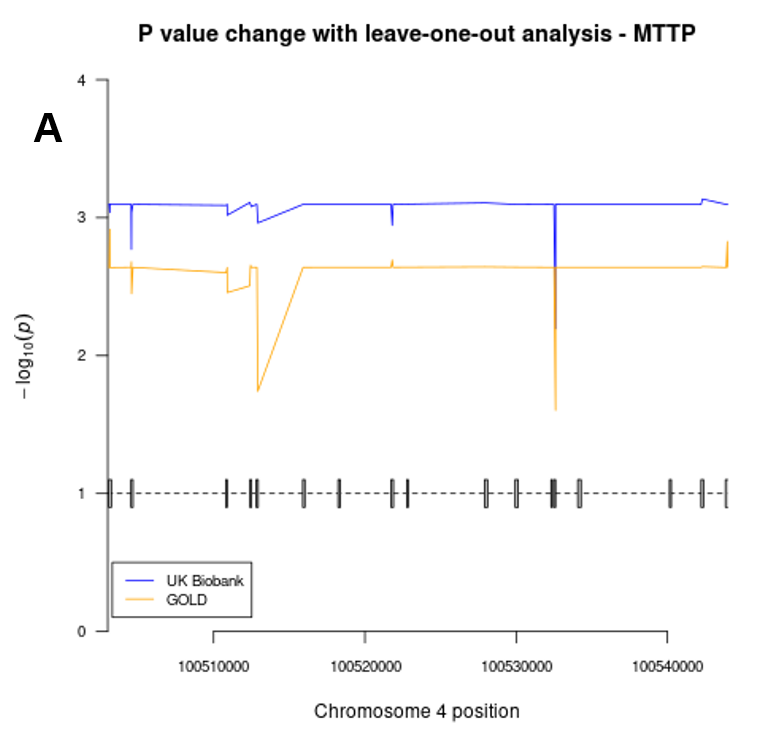
\includegraphics[width=0.7\linewidth]{"images/fig2.png"} 
  \caption{\textbf{Leave One Variant Out plot} (from Du et al 2021). Vertical drops signify associated single variants. V's signify regions of associating rare variants}
  \label{fig:f2}
\end{figure}
  

We can then apply any peak-finding algorithm (like golden search or derivative approaches) to identify which variants resulted in large peaks of association signal change. This will help identify if the effects of the protein-altering variants are restricted to a specific region of the gene or not. we can then isolate specific regions of a gene and potential polypeptide sequences to study for follow-up analysis.

To verify that we have identified specific causal locations within a gene we can construct a gene-based test using only our implicated causal locations and identifying if the association improves or gets worse. If we do identify a singular causal region we expect the gene-based association p-value to improve. If the causal region of the gene cannot be well defined then we expect the gene-based association to perform worse.

We expect to have a list of genomic endpoints for each gene implicating the deleterious or important parts of a gene relating to MetS. If we cannot identify a single causal region then the endpoints should encapsulate the entire gene.

\subsection*{Aim 2b: Design CRISPR CAS9 KO guides based on exonic variants.} 

If the variants lie in the exons of a gene and result in a missense or loss-of-function mutation, we can even simulate the folded mutated protein using AlphaFold2 to assess hydrophobic and hydrophilic region changes across the proteins helping inform future functional studies for potential assays and tests to run with these results.

There are a plethora of tools for single-guide RNA (sgRNA) design for gene knockout experiments such as CRISPOR or CHOPCHOP, and we can use them to generate a list of potential gene knockout guides for each implicated gene.

Then for the genes from 2a of whom we were able to identify specific within gene sequences, we can further filter and assess the recommended guides to help build a more focused MetS gene knockout library.

The benefit of this library compared to a standard gene knockout library is the added ability to conduct partial knockouts to study not only the effect of gene omission but a targeted region-specific mutation of a MetS-implicated gene.

Finally, we expect to receive a set of sequences for each MetS-implicated gene that can directly be applied to a functional study of MetS for an in-vitro model.


\subsection*{Potential Outcomes and Conclusions}

We expect to have identified a few new genes implicated to MetS through exonic rare variants along with a suite of sgRNA guides for follow-up CAS9 KO functional experiments. 

However, due to the feed-forward nature of the study in which current results depend on previous results, we could fail to implicate any genes with MetS from Aim 1. In the case this happens we can Meta-Analysze UKBB and MGI together omitting the validation in an independent dataset step. We can make use of newer techniques such as MetaSTAAR which allows for gene-based meta-analysis.

Another limitation of the study is that the annotation of the variants greatly influences the gene-based results. If a variant is annotated to be loss-of-function, we assume that those types of variants have stronger effects compared to missense or synonymous variants. However, there may be regulatory functions in the body that can identify deleterious mutations and suppress gene expression of them negating their potential phenotypic effect. RefGene is a reputable resource however due to the many gaps in our understanding of biology its annotations may not be complete. If our implicated MetS genes are strange or don't validate with previous studies we might try different annotation methods for variants. A recent annotation method tool called FAVOR which makes use of more variant features might be able to address some of those weaknesses.


\newpage

\bibliography{proposal} 
\bibliographystyle{ieeetr}

\end{document}